\section{アンカーの発話区間検出実験}
\label{chapter:get_anchor}

\subsection{実験条件}
同一話者の可能性が高い発話区間を結合し、結合した発話区間を用いてi-vectorを再抽出した。次に、再抽出したi-vectorを用いてアンカーの発話区間検出を行った。発話区間の結合手法は以下の通りである。

\begin{itemize}
\item 手法1 : 発話の間隔情報を考慮して発話区間の結合する
\item 手法2 : 発話環境を考慮して発話区間の結合する
\item 手法3 : 手法1 + 手法2
\end{itemize}

各手法を用いて結合した発話データからi-vectorを抽出し、抽出したi-vectorを用いてアンカーの発話区間検出を行う。アンカーの発話区間検出手法は\ref{section:clustering}節の手法を用いる。また、Baselineとして、音源分離によって得られた発話区間から得られたi-vectorを用いたアンカーの発話区間検出を行う。


前後の発話区間を結合する際のi-vectorのコサイン類似度の閾値を表\ref{table:decide_thcos}に示す。ここで、$T$は発話区間の秒数である。これは、図\ref{fig:same_cos_hist}で示されるように、同一話者間の発話であっても発話の長さによってコサイン類似度の値が大きく異なり、図\ref{fig:same_cos_vari}で示されるように発話が短い時、同一話者間のi-vectorのコサイン類似度の標準偏差が非常に大きいためである。そのため、本実験では、3.5秒と7秒で閾値を変更し、発話区間の結合に用いた。

\begin{table}[H]
  \begin{center}
    \caption{発話区間の結合の閾値 \label{table:decide_thcos}}
    \begin{tabular}{|c||c|} \hline
時間条件 & コサイン類似度の閾値  \\ \hline
$T <$ 3.5 &  0.2 \\ \hline
3.5 $\leqq T <$ 7 &  0.6  \\ \hline
7 $\leqq T$ &  0.75 \\ \hline
    \end{tabular}
  \end{center}
\end{table}

手法1、および手法3で用いる非発話区間の長さの閾値$Th_{time}$を0.8秒から1.5秒までの範囲を0.1秒刻みで、i-vectorを用いたアンカーの発話区間検出におけるアンカーか否かを判別する$Th_{cos}$を0.5から0.8までの範囲を0.1刻みで変更して実験を行う。\par
i-vectorの抽出には、ALIZEとLIR RALを用いる。i-vectorの抽出に使用するUBMモデルの学習には読み上げ音声\cite{ATR}を使用する。読み上げ音声に収録されている各発話データからi-vectorを抽出する。発話データから抽出する音響特徴パラメータを表\ref{iv_feature2}に示す。また混合数は32とした。\par

\begin{table}[H]
  \begin{center}
    \caption{使用する音響特徴パラメータ \label{iv_feature2}}
    \begin{tabular}{|c||c|} \hline
      特徴量 & 次元数\\ \hline
      MFCC & 19  \\ 
      POW & 1  \\ 
      $\Delta$MFCC & 19 \\ 
      $\Delta$POW & 1 \\ 
      $\Delta\Delta$MFCC & 19 \\ 
      $\Delta\Delta$POW & 1 \\ \hline
      計 & 60 \\ \hline
    \end{tabular}
  \end{center}
\end{table}

\subsection{評価方法}
評価は、検出されたアンカーの発話区間と正解ラベルを比較して行う。

\begin{table}[H]
\begin{center}
    \caption{アンカーの発話区間の正誤判定 \label{table:clustering}}
\begin{tabular}{|c|c|c|c|l}
\cline{1-4}
\multicolumn{2}{|c|}{\multirow{2}{*}{}} & \multicolumn{2}{c|}{「発話者」のラベルが付与された発話区間} &  \\ \cline{3-4}
\multicolumn{2}{|c|}{}                  & アンカーの発話区間        & アンカー以外の発話区間        &  \\ \cline{1-4}
\multirow{2}{*}{判定結果}        & 正        & $TP$                  & $FP$                   &  \\ \cline{2-4}
& 誤        & $FN$                  & $TN$                   &  \\ \cline{1-4}
\end{tabular}
\end{center}
\end{table}

表\ref{table:clustering}に示すアンカーの発話区間の正誤判定を行い、$P$(適合率(Precision))と$R$(再現率(Recall))を式\ref{calc:precision2}と式\ref{calc:recall2}のようにそれぞれ計算する。また、$F$値($F-measure$)を式\ref{calc:fmeasure2}のように計算する。

\begin{equation}
\label{calc:precision2}
P = \frac{TP}{TP + FP}
\end{equation}

\begin{equation}
\label{calc:recall2}
R = \frac{TP}{TP + FN}
\end{equation}

\begin{equation}
\label{calc:fmeasure2}
F = \frac{1}{\frac{1}{P} + \frac{1}{R}}
\end{equation}

ここで$P$と$R$はそれぞれ適合率、再現率を表す。

また、検出したアンカーの発話区間の割合を式\ref{calc:anchor_acc}を用いて評価する。

\begin{equation}
\label{calc:anchor_acc}
Acc_{time} = \frac{検出したアンカーの発話区間の時間数}{アンカーの発話区間の時間数}
\end{equation}

本実験では、評価方法として適合率、再現率、$F$値、$Acc_{time}$を用いる。

\subsection{実験結果}
アンカーの発話区間検出精度を図\ref{fig:result_anchor_baseline} $\sim$ 図\ref{fig:result_anchor_prob3}に示す。本節では各手法で最も良いF値を示した条件の結果を記載している。その他の条件の結果は付録で記載する。

\begin{figure}[H]
  \begin{center}
    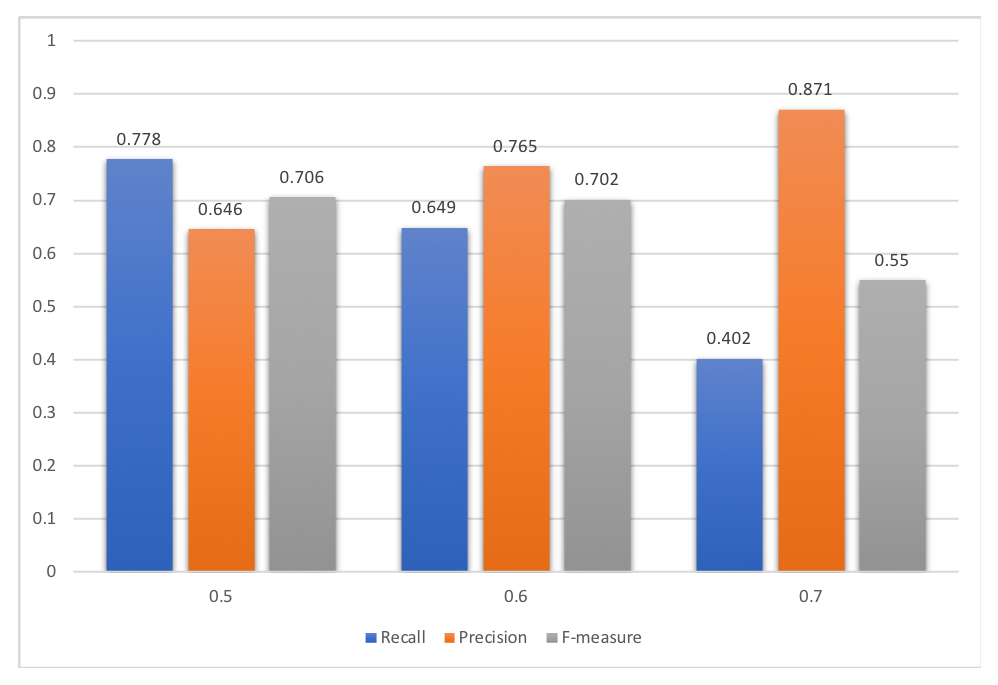
\includegraphics[scale=0.8]{./figure/get_anchor_baseline.eps}
  \end{center}
  \caption{Baselineによる発話区間検出精度 \label{fig:result_anchor_baseline}}
\end{figure}

\begin{table}[H]
  \begin{center}
    \caption{Baselineによる各ニュース番組音声のアンカーの発話区間検出精度($Th_{cos}=0.5$) \label{table:NHK_pause_RPF}}
    \begin{tabular}{|c||c|c|c|c|} \hline
データID & Recall & Precision & F-meature & 作成したクラスタ数\\ \hline
ニュース1 & 0.970 & 0.623 & 0.758 & 1 \\ \hline
ニュース2 & 0.709 & 0.437 & 0.540 & 2 \\ \hline
ニュース3 & 0.736 & 0.719 & 0.727 & 2 \\ \hline
ニュース4 & 0.728 & 0.661 & 0.693 & 2 \\ \hline
ニュース5 & 0.683 & 0.947 & 0.793 & 2 \\ \hline
    \end{tabular}
  \end{center}
\end{table}

\begin{figure}[H]
  \begin{center}
    \includegraphics[scale=0.8]{./figure/get_anchor_prob1.eps}
  \end{center}
  \caption{手法1によるアンカーの発話区間検出精度 ($Th_{time}=1.2$) \label{fig:result_anchor_prob1}}
\end{figure}

\begin{table}[H]
  \begin{center}
    \caption{手法1による各ニュース番組音声のアンカーの発話区間検出精度($Th_{cos}=0.6,Th_{time}=1.2$) \label{table:NHK_pause_RPF}}
    \begin{tabular}{|c||c|c|c|c|} \hline
データID & Recall & Precision & F-meature & 作成したクラスタ数\\ \hline
ニュース1 & 0.964 & 0.707 & 0.815 & 1 \\ \hline
ニュース2 & 0.764 & 0.685 & 0.722 & 3 \\ \hline
ニュース3 & 0.729 & 0.860 & 0.789 & 2 \\ \hline
ニュース4 & 0.683 & 0.741 & 0.711 & 2 \\ \hline
ニュース5 & 0.695 & 0.978 & 0.813 & 2 \\ \hline
    \end{tabular}
  \end{center}
\end{table}

\begin{figure}[H]
  \begin{center}
    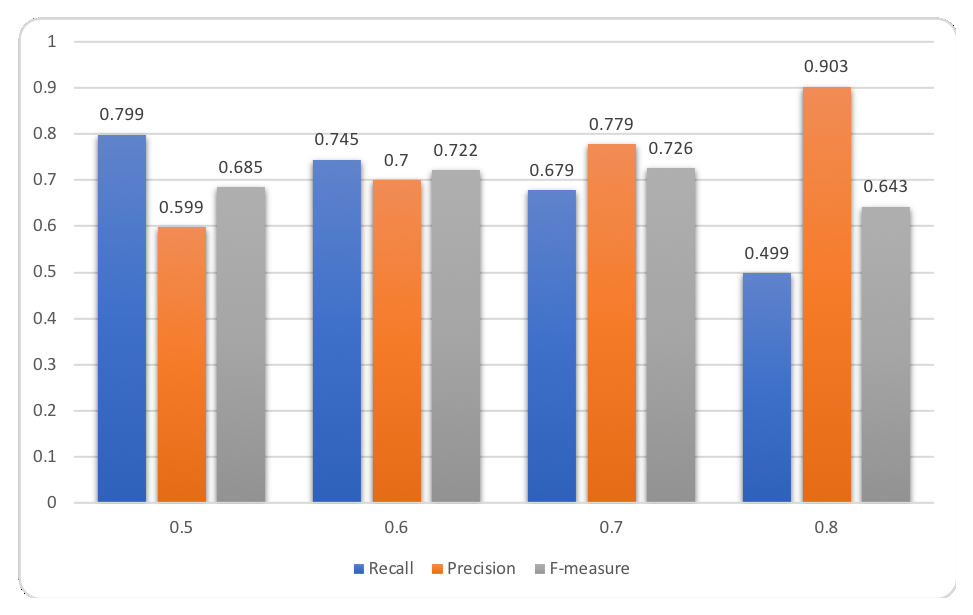
\includegraphics[scale=0.8]{./figure/get_anchor_prob2.eps}
  \end{center}
  \caption{手法2によるアンカーの発話区間検出精度 \label{fig:result_anchor_prob2}}
\end{figure}

\begin{table}[H]
  \begin{center}
    \caption{手法2による各ニュース番組音声のアンカーの発話区間検出精度($Th_{cos}=0.6$) \label{table:NHK_pause_RPF}}
    \begin{tabular}{|c||c|c|c|c|} \hline
データID & Recall & Precision & F-meature & 作成したクラスタ数\\ \hline
ニュース1 & 0.958 & 0.617 & 0.751 & 1 \\ \hline
ニュース2 & 0.788 & 0.512 & 0.621 & 2 \\ \hline
ニュース3 & 0.695 & 0.823 & 0.754 & 2 \\ \hline
ニュース4 & 0.683 & 0.732 & 0.707 & 2 \\ \hline
ニュース5 & 0.679 & 0.960 & 0.796 & 2 \\ \hline
    \end{tabular}
  \end{center}
\end{table}

\begin{figure}[H]
  \begin{center}
    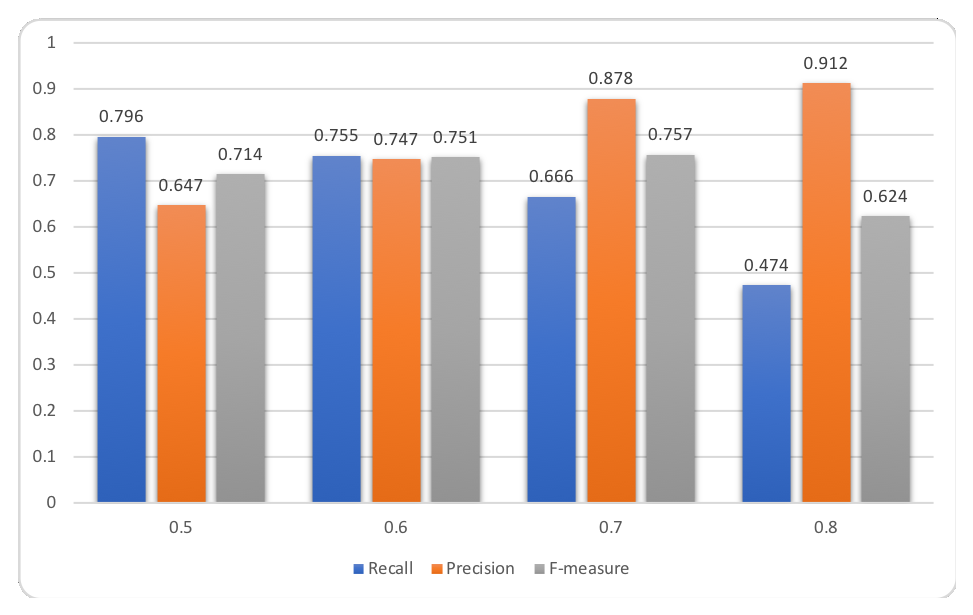
\includegraphics[scale=0.8]{./figure/get_anchor_prob3.eps}
  \end{center}
  \caption{手法3によるアンカーの発話区間検出精度 ($Th_{time}=1.3$) \label{fig:result_anchor_prob3}}
\end{figure}

\begin{table}[H]
  \begin{center}
    \caption{手法3による各ニュース番組音声のアンカーの発話区間検出精度($Th_{cos}=0.6,Th_{time}=1.3$) \label{table:NHK_pause_RPF}}
    \begin{tabular}{|c||c|c|c|c|} \hline
データID & Recall & Precision & F-meature & 作成したクラスタ数\\ \hline
ニュース1 & 0.958 & 0.702 & 0.810 & 1 \\ \hline
ニュース2 & 0.758 & 0.590 & 0.663 & 2 \\ \hline
ニュース3 & 0.725 & 0.846 & 0.781 & 2 \\ \hline
ニュース4 & 0.646 & 0.755 & 0.696 & 2 \\ \hline
ニュース5 & 0.683 & 0.973 & 0.802 & 2 \\ \hline
    \end{tabular}
  \end{center}
\end{table}

実験の結果、発話区間を結合して再抽出したi-vectorを用いた手法が全体的に高い精度を示した。Baselineは$Th_{cos}$が0.8のときアンカーの発話区間を検出できなかった。また、Baselineは$Th_{cos}$が0.5のときがF-measureが最も高い値をとるのに対して、本提案手法では$Th_{cos}$が0.6のとき、F-measureが最も高い値をとった。\par
本実験の提案手法では、手法1が最も発話区間検出精度が高く、F値が0.772であった。また、いずれの手法においても$Th_{cos}$が小さい時にはRecallが高く、大きい時にはPrecisionが高くなる傾向が確認された。

\subsection{考察}
Baselineと再抽出したi-vectorを用いた各提案手法を比較したときアンカーの発話区間検出精度が向上したことから、従来と比較してi-vectorが話者の特徴をより抽出できたと考えられる。また、いずれの手法でもニュース2はアンカーの発話区間検出の精度が他のニュースと比較して低い。これは、ニュース2のアンカーの発話数と天気アナウンサーの発話数が影響していると考えられる。ニュース2の2人のアンカーのうち、一人は27発話、天気アナウンサーは36発話であった。よって、天気アナウンサーをアンカーとして認識したことによりP値が低下し、結果として検出精度が低下したと考えらえる。これに関連して、Baselineでアンカーとして検出したクラスタ数は2であったが、そのうち一つはアンカーではなく天気アナウンサーの発話のクラスタとなっており、正確なアンカーの発話のクラスタリング、発話区間検出ができたとは言えない。対して、手法1に関してはアンカーとして検出したクラスタ数が3となっているが、発話数が少ないアンカーの検出にも成功している。しかし、こちらも天気アナウンサーの発話をアンカーとして誤識別しているため、さらなるアンカーの発話区間の検出精度向上には天気アナウンサーの発話か否かを識別する手法が必要であると考えられる。\par
また、手法1 $\sim$